\section{Modular Learning}
\begin{itemize}
	\item \textit{Definition}: A family of \textcolor{green}{parametric}, \textcolor{lightred}{non-linear} and \textcolor{blue}{hierarchical} \textcolor{orange}{representation learning functions}, which are \textcolor{red}{massively optimized with stochastic gradient descent} to \textcolor{purple}{encode domain knowledge}, i.e. domain invariances, stationarity.
	% \item Although with two-layer (shallow) network, we can approximate all possible functions, a deep architecture tends to be more efficient and generalize better
	\item A neural network is a series of hierarchically connected functions $\Rightarrow$ Directed Acyclic graph
	\item Note that it is not allowed to have loops except over time/additional dimension
\end{itemize}
\begin{figure}[ht!]
	\centering
	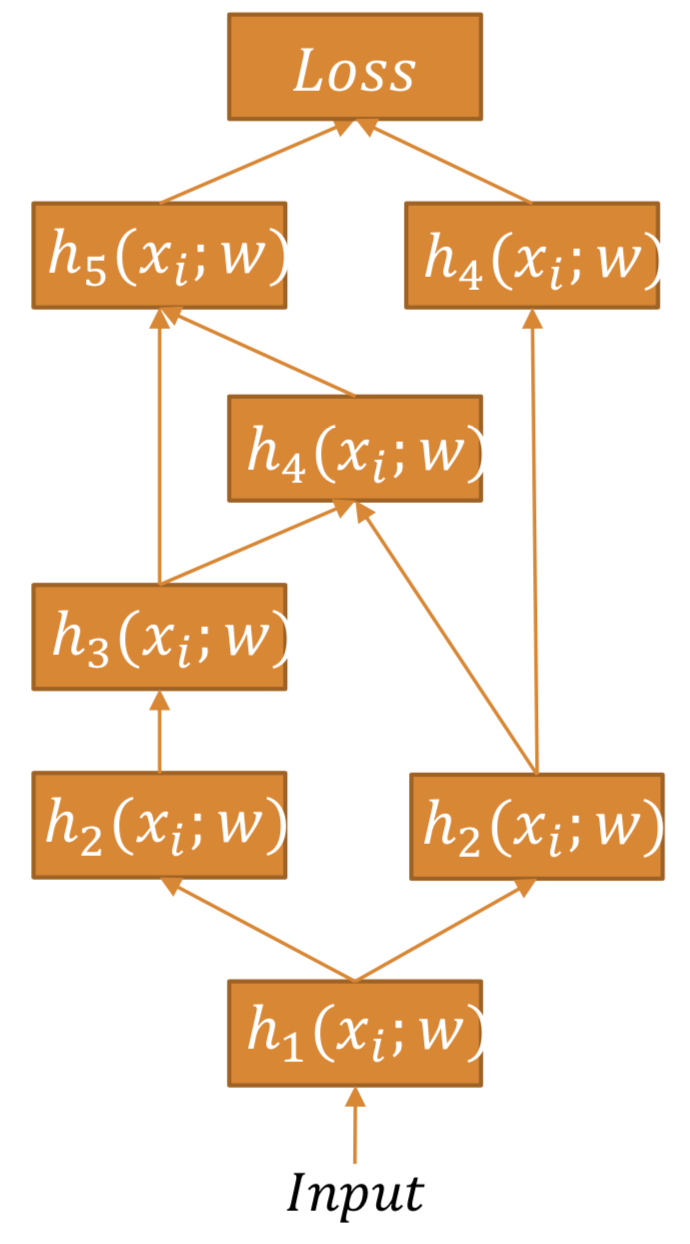
\includegraphics[width=0.2\textwidth]{figures/modularity_example_network.png}
	\caption{Example network with interweaved connections. The architecture can be made arbitrarily complex, and can also include recurrent connections.}
	\label{fig:modularity_example_network}
\end{figure}
\subsection{Module}
\begin{itemize}
	\item A module is the simplest mathematical component in a NN, and can be expressed by $a=h(x;w)$ where $a$ is the output, $x$ the input, $w$ trainable parameters and $h$ an activation function
	\item $w$ mostly learned by gradient-based methods, usually maximizing the likelihood
	\begin{itemize}
		\item ML solution: $w^{*} = \arg\max\limits_{w}\prod\limits_{x,y}p_{model}\left(y|x;w\right)$
		\item For gradient-based methods, we can minimize the negative log likelihood:\\ $\mathcal{L}(w) = -\mathbb{E}_{x,y\sim \tilde{p}_{data}}\left[\log p_{model}\left(y|x;w\right)\right]$
		\item If output is Gaussian, we would get the $\ell_2$ norm
		\item If output is Laplacian, we would get the $\ell_1$ norm
	\end{itemize} 
	\item Using a loss function that matches the output distribution of the network helps, because:
	\begin{itemize}
		\item It makes math simpler (exponential cancels out)
		\item Better numerical stability ($\log$ with very small/negative values, helps for e.g. Softmax+CrossEntropy)
		\item Makes gradients larger as exponential-like activations often lead to saturation, which means gradients are almost 0 (but not with $\log$)
	\end{itemize}
	\item It is important that the input and output distribution of every module match, as otherwise we get inconsistent behavior and makes it harder to learn
	\begin{itemize}
		\item For activation functions, this means we prefer them to be mostly activated around the origin and centered
		\item Otherwise, e.g. ReLU can be come a linear unit or set everything to 0
	\end{itemize}
\end{itemize}
\subsubsection{Example modules}
\begin{itemize}
	\item \textbf{Linear module}: $a = wx$
	\begin{itemize}
		\item Simple gradients $\frac{\partial a}{\partial w} = x$, $\frac{\partial a}{\partial x} = w$
		\item No activation saturation $\Rightarrow$ strong, reliable gradients
	\end{itemize}
	\item \textbf{Rectified Linear Unit}: $a = \max(0,x)$
	\begin{itemize}
		\item Gradient is step function. $\pd{a}{x} = \begin{cases}
		0 & \text{ if } x\leq 0\\
		1 & \text{ if } x > 0\\
		\end{cases}$
		\item Hence, strong, fast gradients
		\item However, dead neurons might be an issue when initialization/weights produce outputs smaller 0 for every input 
		\item Different variations like LeakyReLU, Softplus ($\ln(1+e^{x})$), NoisyReLU exist
	\end{itemize}
	\item \textbf{Sigmoid}: $a=\sigma(x)=\frac{1}{1+e^{-x}}$
	\begin{itemize}
		\item Gradient easy to calculate: $\pd{a}{x} = \sigma(x)\left(1-\sigma\left(x\right)\right)$
		\item Can be used as output function for probability distribution between $[0,1]$
		\item Saturates and has small gradients
		\item Not centered around origin $\Rightarrow$ not good choice for within a network
	\end{itemize}
	\item \textbf{Tanh}: $a=\tanh\left(x\right)=\frac{e^{x}-e^{-x}}{e^{x}+e^{-x}}$
	\begin{itemize}
		\item Gradients $\pd{a}{x}=1-\tanh\left(x\right)^2$
		\item Saturates as well, but has slightly higher gradients than sigmoid and is centered around origin
	\end{itemize}
	\item \textbf{Softmax}: $a^{(k)} = \text{softmax}\left(x^{(k)}\right) = \frac{e^{x^{(k)}}}{\sum_j e^{x^{(j)}}}$
	\begin{itemize}
		\item Probability distribution over multiple classes
		\item Softmax trick for numerical stability: $\frac{e^{x^{(k)}-\mu}}{\sum_j e^{x^{(j)}-\mu}}$
	\end{itemize}
\end{itemize}
\subsection{Backpropagation}
\begin{itemize}
	\item Calculate gradients of all parameters in the network based on the loss on the last layer
	\item Principle of chain rule: $\pd{z}{x} = \sum_j \chain{z}{y_i}{x}$ (gradients from all possible paths)
	\begin{itemize}
		\item In vector notation: $\nabla_{\bm{x}} \bm{z} = \left(\pd{\bm{y}}{\bm{x}}\right)^T \cdot \nabla_{\bm{y}} \bm{z}$ with Jacobian $\pd{\bm{y}}{\bm{x}} = \left[\begin{array}{ccc}
		\pd{y_1}{x_1} & \pd{y_1}{x_2} & \pd{y_1}{x_3} \\[5pt]
		\pd{y_2}{x_1} & \pd{y_2}{x_2} & \pd{y_2}{x_3} \\
		\end{array}\right]$
	\end{itemize}
	\item Steps of Backpropagation:
	\begin{enumerate}
		\item Compute forward propagations for all layers recursively:
		$a^{(l)} = h^{(l)}\left(x^{(l)}\right) \text{ and } x^{(l+1)} = a^{(l)}$
		\item Compute the reverse path. 
		$$\pd{\mathcal{L}}{a^{(l)}} = \left(\pd{a^{(l+1)}}{x^{(l+1)}}\right)^T \cdot \pd{\mathcal{L}}{a^{(l+1)}}, \hspace{4mm} \pd{\mathcal{L}}{\theta^{(l)}} = \pd{a^{(l)}}{\theta^{(l)}} \cdot \left(\pd{\mathcal{L}}{a^{(l)}}\right)^T$$
		\item Use gradients $\pd{\mathcal{L}}{\theta^{(l)}}$ to update parameters via SGD
	\end{enumerate}
\end{itemize}